\section{Market Model}

\begin{figure}[h!]
  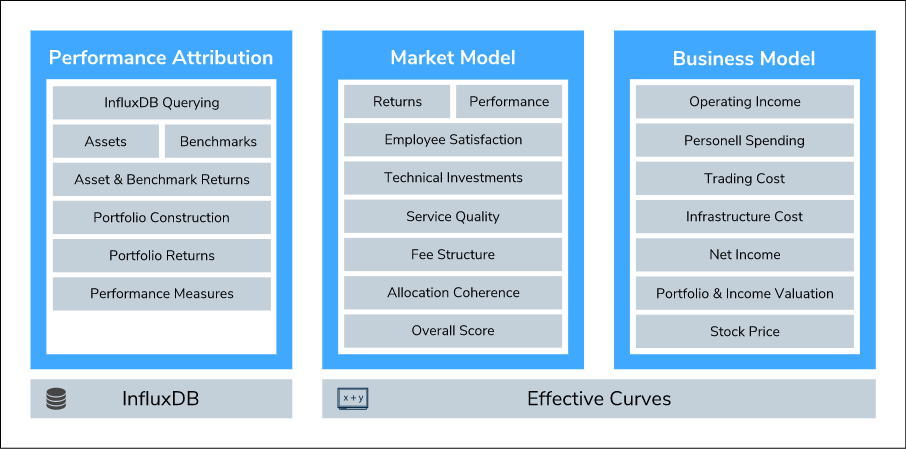
\includegraphics[width=\textwidth]{img/market_model.png}
  \caption{Market Model Overview}
  \centering
  \label{fig:market_model_overview}
\end{figure}

The PFM-Game market model is a module that produces period results based on the business decisions and portfolio allocations of teams participating in a given game. During the execution of a game, the market model is executed once per period once the game master decides to complete a period and send a period scoring request. The market model is separated into several subcomponents that then, when applied in sequence, produce results for the given period of the game.

\subsection{Data and Data Ingestion}
The underlying data driving all portfolio-related calculations in the market model is comprised of several hunderd time-series that are stored in InfluxDB, a database specialized in time-series management. The majority of these time-series describe asset price or return indices (i.e., asset prices normalized by the payment of dividends and other interest) as extracted from the Thomson Reuters Datastream platform. Further relevant time-series are based on macroeconomic data extracted from the FRED (Federal Reserve Economic Data) database. These data are used to calculate portfolio and benchmark returns as well as parameters of an economic forecast.

The above described data can be extracted from Datastream and FRED and ingested into an instance of InfluxDB automatically by means of a Python module that was created as an extension to the \textit{PFM-Simulation} project. Data to be ingested is defined inside an assets.csv file in the following CSV format:

\begin{table}[h!]
  \begin{tabular}{lllllll}
    \toprule
    Name & Symbol  & Start Date & Market      & Data Type & Asset Type & Currency \\
    \midrule
    SWISS BOND AAA & SWBND3A & 29.12.2006 & Switzerland & RI        & BONDS      & CHF      \\
    NESTLE 'R'     & S:NESN  & 01.01.1973 & Switzerland & RI        & EQUITY     & CHF      \\
    \bottomrule
  \end{tabular}
  \centering
  \caption{Exemplary assets in a valid assets.csv definition format (optional columns omitted)}
  \label{table:assets_csv}
\end{table}

During processing of the CSV definition of all assets, the module will incrementally extend existing time-series with new data up to the current day. Time-series that were not previously available will be stored as a new series in full-length. As not all assets are available at all times, the game will dynamically decide about the assets to show as potential investments based on their availability and the historical dates of the period.


\subsection{Performance Attribution}
The performance attribution module is the first module in the sequence of model calculations that are applied to an incoming period scoring request. This module handles everything from extracting the relevant time-series from the database to computing key performance measures on constructed portfolios.

% modules/performance_attribution/influx.py
\subsubsection{InfluxDB Querying}
As can be seen in \ref{fig:market_model_overview}, one of the most important responsibilities of the performance attribution module is handling all data querying from the InfluxDB time-series database. Based on the incoming depot allocations of teams that participate in a game, the module fetches all necessary asset and benchmark series from the database. \footnote{See pfm-model/api/modules/performance\_attribution/influx.py}

% modules/performance_attribution/returns.py
\subsubsection{Asset \& Benchmark Returns}
To be able to continue with portfolio construction further in the sequence, all extracted time-series need to be converted into series of returns. All computations later in the sequence will be based on these relative return measures and not on any absolute values of the time-series.\footnote{See pfm-model/api/modules/performance\_attribution/returns.py}

% modules/performance_attribution/portfolio.py
\subsubsection{Portfolio Construction}
With returns being available for all assets and their corresponding benchmarks, the performance attribution module then constructs portfolios for each team. Each team will have created one portfolio allocation for each customer type that is enabled for a specific period. The module will account for this by constructing as many portfolios per team as there are customer types.\footnote{See pfm-model/api/modules/performance\_attribution/portfolio.py}

In addition to building portfolios for all depot allocations of the current period, the performance attribution module also computes a benchmark portfolio for each asset portfolio. These benchmark portfolios are based on the strategic asset allocation of the corresponding team and customer type. As the strategic asset allocation is defined once per game (during period zero), the composition (but not the returns) of these benchmark portfolios stays the same over the course of the entire game.

% modules/performance_attribution/returns.py
\subsubsection{Portfolio Returns}
Once portfolios have been built for each combination of teams and active customer types, returns need to be calculated in the same way that returns were calculated for the assets previously. To compute a portfolio return, the separate asset returns need to be weighted by the amount of money that has been invested into each asset. For example, if a team were to invest 10\% of their total assets under management in one asset and 20\% in another, the latter would influence the overall portfolio returns twice as much as the former.

% modules/performance_attribution/kpi.py
\subsubsection{Performance Measures}
Upon completion of all previous returns calculations, the returns of assets, benchmarks, and portfolios can be combined into many useful performance measures that characterize a portfolio in different ways and allow for an easy performance comparison between teams. \ref{table:portfolio_measures} provides an overview over all of the measures made available by the performance attribution module.

\begin{table}[h!]
    \begin{tabular}{ll}
      \toprule
      Name & Description \\
      \midrule
      Variance     & The variance of portfolio returns \\
      Standard Deviation     & The standard deviation of portfolio returns \\
      Variance BM & The variance of a benchmark portfolio \\
      Standard Deviation BM & The standard deviation of a benchmark portfolio \\
      Beta & Systematic risk (volatility) of a portfolio compared to the overall market \\
      Tracking Error     & Divergence between the price behavior of a portfolio and its benchmark \\
      Sharpe Ratio     & Excess return per unit of total risk \\
      Traynor Ratio     & Excess return per unit of systematic risk \\
      Jensen's Alpha     & Difference between portfolio return and expected return according to the Capital Asset Pricing Model (CAPM) \\
      Information Ratio     & Measures abnormal return that could be diversified away by holding an index portfolio \\
      Selection Performance Attribution & Portfolio performance attributed to the individual investments \\
      Tactical Performance Attribution & Portfolio performance attributed to the asset allocation (asset types and markets) \\
      SAA Violations     & The number of times that an ideal SAA has been violated by a given portfolio \\
      TAA Discrepancy     & The relative deviation of a given portfolio with respect to its corresponding TAA \\
      \bottomrule
    \end{tabular}
    \centering
    \caption{Portfolio measures as calculated in the performance attribution module.}
    \label{table:portfolio_measures}
  \end{table}

A byproduct of these calculations are the new assets under management for a customer given their portfolio returns, as well as the new asset positions that a portfolio is composed of after application of returns. For example, if one team invested 50\% in one asset and 50\% in another, the new positions after returns might be 45\%-55\% if the latter asset outperforms the former.\footnote{See pfm-model/api/modules/performance\_attribution/kpi.py}

\subsubsection{Major Outputs}
The results of the performance attribution module are then compiled into a suitable format and passed on to the market model module, which handles the integration of these results with business decisions as well as the grading of performance measures according to efficient curves.


\subsection{Market Model}
The market model module is the second module in the sequence of calculations and builds upon the results of the performance attribution module. It ingests these results as well as business decisions of all teams for the current period and performs several grading procedures based on all of these data. The final output of the module are several index and subindex values that, e.g., describe the employee satisfaction on a range from 0 to 10. The market model module is based on the Excel formulation created by the DBF and was extended by the ability to handle multiple customer types as well as integration with the other modules.

As the market model is comprised of many individual calculation steps and formulas, we will not go deeply into technical specifics of single formulas. Instead, we focus on the overall structure of the module and its main subcomponents as well as how the underlying effective curves (i.e., formulas) can be parametrized and fine-tuned.

\subsubsection{Effective Curves}
To facilitate the grading of arbitrary values on a scale of zero to ten and allow for additional parametrization, formulas that we call effective curves are applied. These formulas most often follow the general schema of computing the market average and, based on a comparison with specific portfolio-related values (\(\Delta = value - value_{avg}\)), calculating a positive or negative deviation from a base value (e.g., \(5 + \Delta \)).

A simple example for an effective curve could be:
\[\text{index value} = 5 + \frac{\Delta}{20000}\]

where the value would be constrained to lie within \([0, 10]\). More complex variants apply different functions based on the domain of the delta value. As a specific example, the full returns index is computed as follows (if the delta value is positive):
\[\text{returns index} = 5 + \log(1 + 10 * |(return - return_{avg}) * 100|)\]

If the delta were negative, the result of the logarithm would simply be inverted to its negative value.

\paragraph{Parametrization}
To allow for easy parametrization of the effective curves, they have been extracted into a single file as lambda functions. An example for such a function is the salary index that takes in a list of salaries and computes the salary index for each one of them:

ix_salary = lambda salary: utils.ensure_index_borders(
    (salary - salary.mean()) / 20000 + 5
)

\subsubsection{Overview of Market Model Indices}
The market model encompasses many calculations and intermediary values. \ref{fig:market_model_dependencies} shows the dependencies and interconnections between all these values, as well as how the final score index and number of customers are calculated. \ref{table:market_model_indices} shortly describes each major index and its significance.

\begin{figure}[h!]
  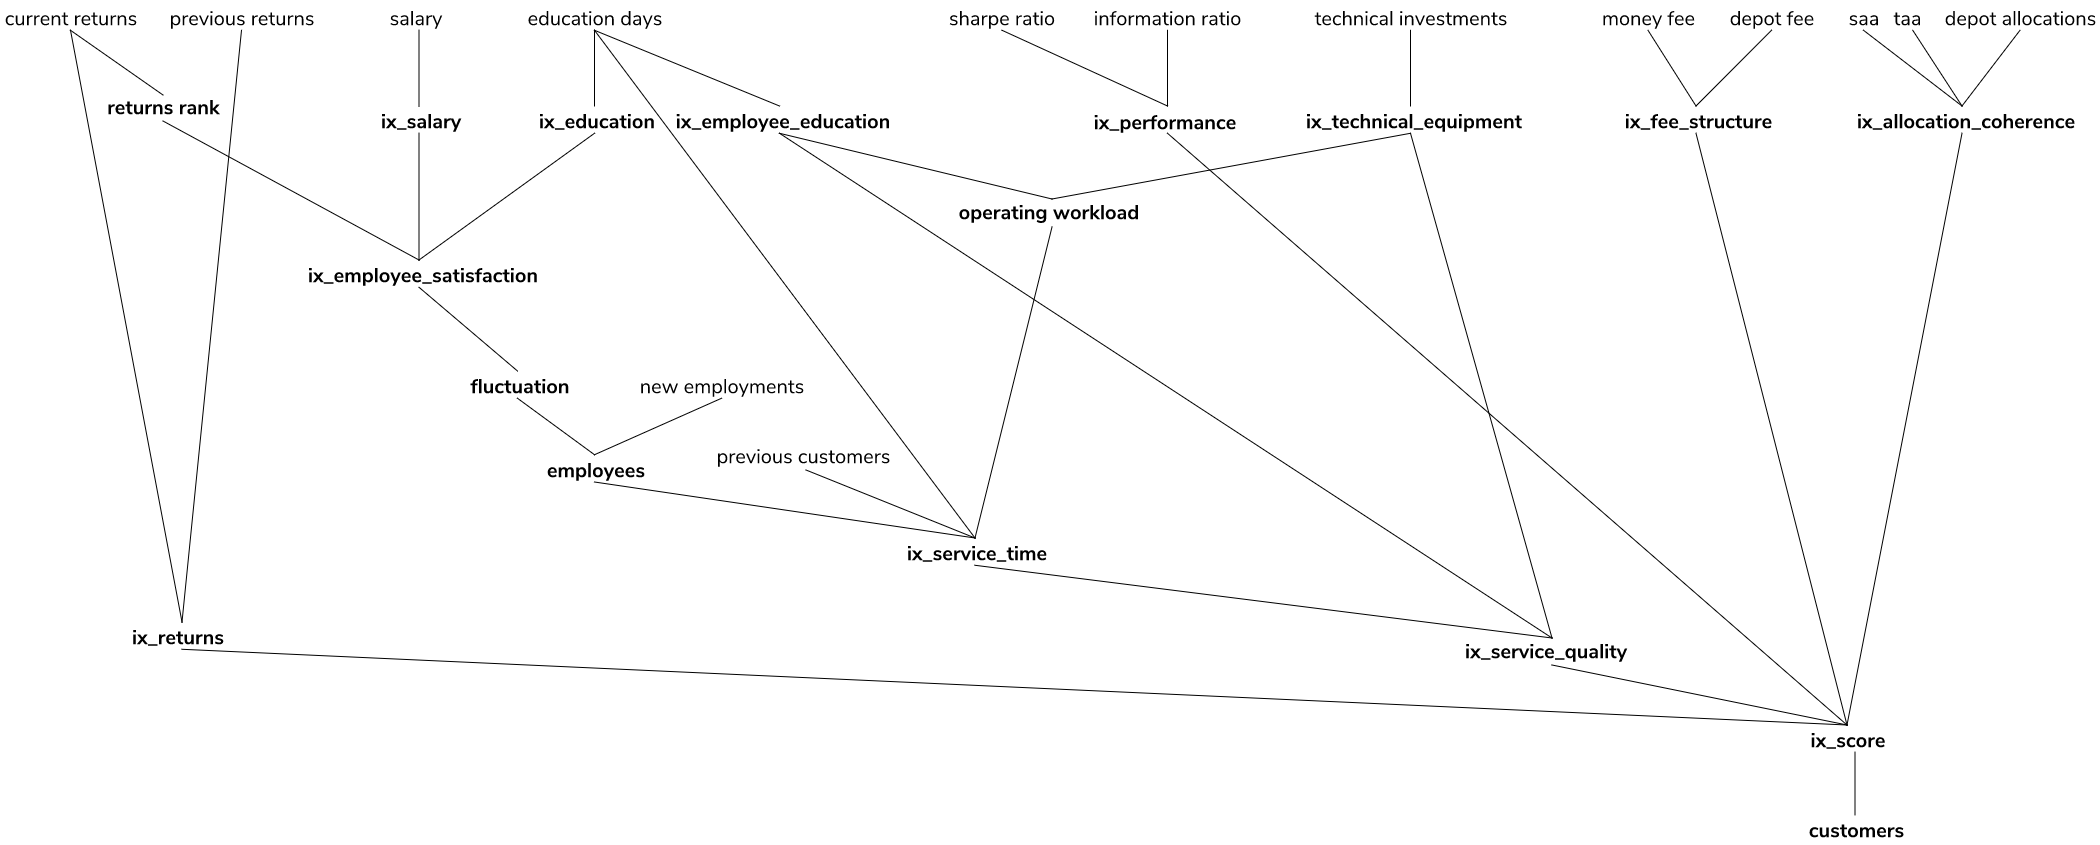
\includegraphics[width=\textwidth]{img/market_model_dependencies.png}
  \caption{Market Model Dependencies}
  \centering
  \label{fig:market_model_dependencies}
\end{figure}

\begin{table}[h!]
  \begin{tabular}{lp{11cm}}
    \toprule
    Name & Description \\
    \midrule
    ix\_returns & How portfolio returns compare against competitors \\
    \midrule
    ix\_sharpe\_ratio & How well the sharpe ratio compares against competitors \\
    ix\_information\_ratio & How the information ratio compares against competitors \\
    ix\_performance & Combination of performance indices \\
    \midrule
    ix\_salary & How satisfied employees are with their salary \\
    ix\_education & How satisfied employees are with their education \\
    ix\_employee\_satisfaction & How satisfied the employees are with overall working conditions \\
    \midrule
    ix\_employee\_education & How much employee education boosts efficiency \\
    ix\_technical\_equipment & How appropriate the IT infrastructure is after depreciation  \\
      ix\_service\_time & How appropriate the time spent for customer service is perceived \\
    ix\_service\_quality & How well overall customer service is perceived \\
    \midrule
    ix\_fee\_structure & How well the all-in management fee is perceived \\
    \midrule
    ix\_allocation\_coherence & Number of SAA violations and relative TAA discrepancy \\
    \midrule
    ix\_score & Combination of all indices into an overall rating \\
    \bottomrule
  \end{tabular}
  \centering
  \caption{Description of all indices calculated in the market model module}
  \label{table:market_model_indices}
\end{table}


\subsubsection{Major Outputs}
Next to the score index encoding the overall satisfaction of customers with a team's bank, it further enables the calculation of customer flows in between teams. Successful teams will earn the customers that other teams lose. The final customer count adjusted by growth will allow for further model calculations regarding overall business income.


\subsection{Business Model}
As the third and final module in the chain, the business model is responsible for all calculations relating to the overall success of a team's banking institution. It calculates a complete income statement with operating returns and expenses as well as equity, dividends, and a final stock price. Next to the number of customers and score index, the stock price serves as the overall score of a team's bank.

\subsubsection{Gross Income}
The gross income of a company includes all revenue earned by goods and services sold. Applied to the scenario of a bank in our game, the gross income can be calculated from the number of customers, assets per customer, and the fee charged for managing said assets. In the case of multiple customer types, the gross income is the sum of all the fees for each separate type.

\subsubsection{Personell Spending}
Personell spending is based on the number of employees and computed by combination with additional factors like salary plus social expenses, education (days per employee), and staffing decisions (hire/fire and temporary staff).

\subsubsection{Trading Cost}
The trading cost of a bank is comprised of a fixed trading cost based on the number of employees as well as a variable trading cost that varies with the number of transactions made by a bank.

\subsubsection{Infrastructure Cost}
A bank's infrastructure cost has two subcomponents: the cost of a workspace needed for each employee and the cost of depreciations on technical investments of previous periods.

\subsubsection{Operating Income and Equity}
The equity of a bank is calculated from the operating income (gross income minus all spending) and the equity of the previous period. Based on the payout ratio as defined by the team, dividends are paid to the bank's shareholders and subtracted from the equity. This equity after dividends will be used as an initial value in the next period.

\subsubsection{Stock Price}
As a final measure, the stock price of a bank measures the confidence of shareholders in the future success of the bank. The calculation is based on the  valuation of all portfolios managed by a bank as well as the valuation of the overall income, equity, and dividends, and the corresponding delta from the previous period.


\subsection{API Specification}


